%auto-ignore
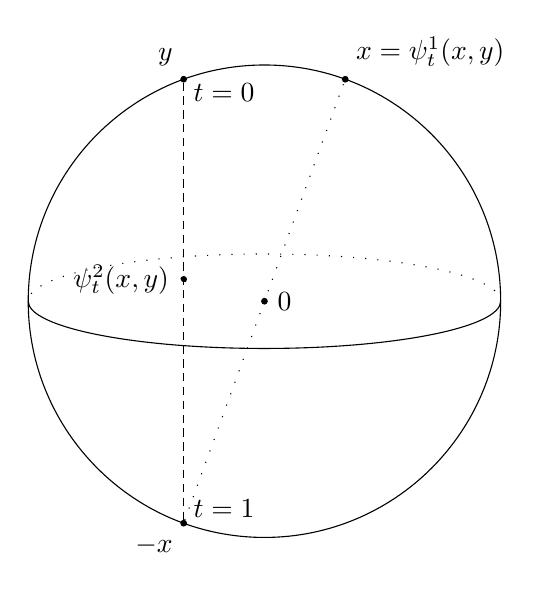
\begin{tikzpicture}
  \tikzset{point/.style = {draw, circle, fill=black, minimum size=2pt,inner sep=0pt}}
  \tikzset{->-/.style={decoration={markings,mark=at position #1 with {\arrow{>}}},postaction={decorate}}}
  \tikzset{-<-/.style={decoration={markings,mark=at position #1 with {\arrow{<}}},postaction={decorate}}}

  \def\rad{3cm}
  \def\posx{70}
  \def\posy{110}
  
  % Sphere
  \node [point,label={0:0}] (C) at (0,0) {};
  \draw (C) circle (\rad);
  \draw (-\rad,0) arc (180:360:3 and 0.6);
  \draw[loosely dotted] (\rad,0) arc (0:180:3 and 0.6);
  
  
  \path (C) node[point,label={\posx:$x=\psi^{1}_t(x,y)$}] (x)  at +(\posx:\rad) {};
  \path (C) node[point,label={\posx+180:$-x$}] (mx)  at +(\posx+180:\rad) {};
  \path (C) node[point,label={\posy:$y$}] (y)  at +(\posy:\rad) {};
  
  \draw[loosely dotted] (mx) -- (x);
  \draw[densely dashed] (y) node [label={[label distance=-6pt,yshift=1pt,xshift=1pt]-50:$t=0$}] {} -- node[point,pos=0.45,label={[left,label distance=-3pt]0:$\psi_t^{2}(x,y)$}] {} (mx) node [label={[label distance=-6pt,yshift=11pt,xshift=1pt]-50:$t=1$}] {};
\end{tikzpicture}